\section{Design}

FlashMatrix is a general-purpose data analysis framework that provides
matrix-oriented programming interface. It provides a set of generalized
vector and matrix operations and supports vector and matrix operations in R.
FlashMatrix supports multiple R data containers and stores these data containers
on SSDs to scale to very large data sets. Like most of R functions,
the operations in FlashMatrix do not change data in the input data containers
and each operation generates a new data container.

\subsection{Architecture}

\begin{figure}
\centering
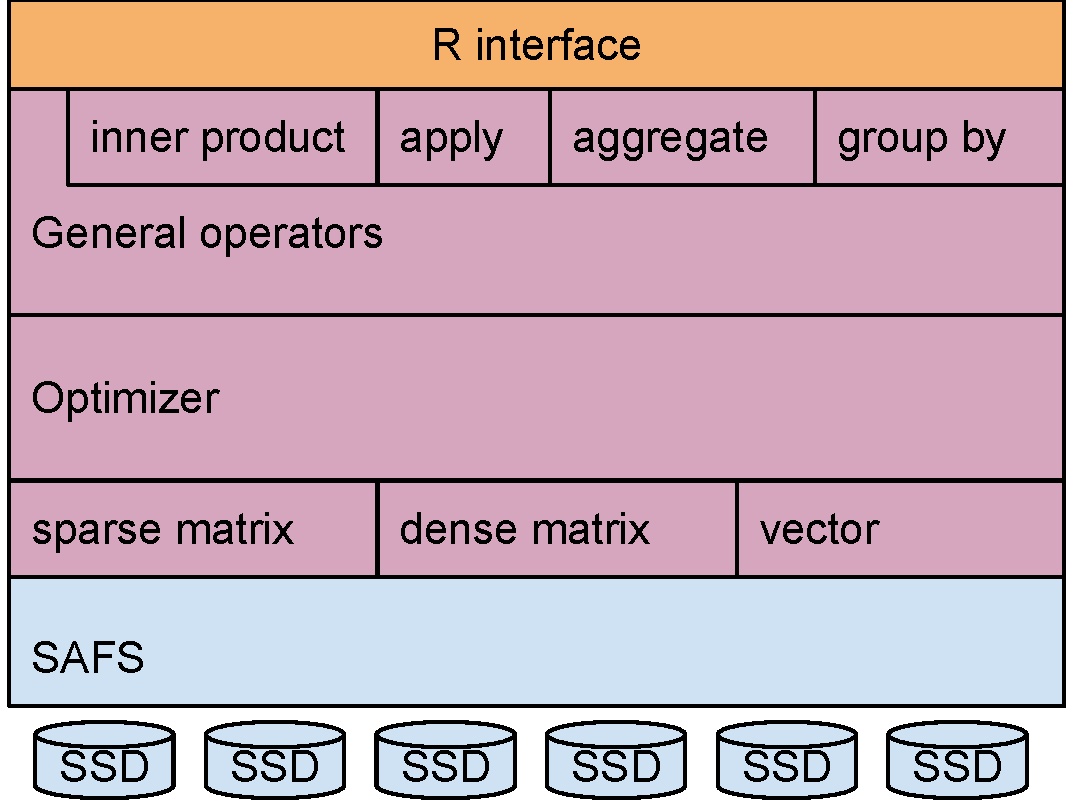
\includegraphics[scale=0.3]{./architecture.pdf}
\vspace{-5pt}
\caption{The architecture of FlashMatrix.}
\vspace{-5pt}
\label{arch}
\end{figure}

\subsection{Data containers}
FlashMatrix supports multiple R data containers. It has two types of basic
data containers: \textit{vector} and \textit{matrix}. In addition, it also
supports two types of more advanced data containers: \textit{vector of vectors}
and \textit{data frame}, constructed from \textit{vector}.
% We need to support sparse vector, set and map.

\begin{itemize}
	\item  A \textit{vector} is a one-dimensional array and each element has
	the same type.
	\item A \textit{matrix} is a two-dimensional array and each element has
	the same type. FlashMatrix supports both row-major and column-major
	matrices. The layout of a matrix is generally determined by a FlashMatrix
	operation but can also be determined by users. FlashMatrix supports both
	dense matrices and sparse matrices.
	\item A \textit{vector of vectors} is a more restricted variant of R
	\textit{list} and requires each vector has the same element type. A row-major
	matrix can be viewed as a special \textit{vector of vectors} with each
	vector of the same length.
	\item A \textit{data frame} is a collection of vectors and each vector can
	have arbitrary element types. All vectors in a data frame has the same length.
	A column-major matrix can be viewed as a data frame with each vector of
	the same element type.
\end{itemize}

Each type of data containers has two variants: local containers and global
containers. A global container stores data on SSDs and supports varieties of
generalized computation operators in Section \ref{sec:generalized}. A local
container is created by a generalized computation operator in a thread and
is exposed to VUDF. To increase data locality, the data in a local container
is stored in memory local to the processor where the thread runs.

%\subsection{Basic operations} \label{sec:basic}
%create a data container

%data container conversion

%matrix operations: convert data layout and transpose.

%append an element to a vector can be implemented as physically appending the element
%to the vector. The result vector becomes the new vector, and the original vector
%becomes the sub-vector of the new vector.

\subsection{Generalized computation operations} \label{sec:generalized}
To enhance the flexibility and simplify the implementation, FlashMatrix only
provides a small set of generalized operators on vectors and matrices.
The current implementation has four generalized operators: \textit{inner product},
\textit{apply}, \textit{aggregation} and \textit{groupby}. Each operator
accepts user-defined functions (UDF).

\textit{Inner product} is a generalized matrix multiplication. It replaces
multiplication and addition in matrix multiplication with two user-defined
functions, respectively. As such, we can define many operations with inner
product. For example, we can use inner product to compute various pair-wise
distance matrics of vectors such as Euclidean distance \cite{euclidean} and
Hamming distance \cite{hamming}. We can also apply inner product to sparse
matrices to compute PageRank, belief propagation, etc.
Even though we can implement matrix multiplication with inner product,
FlashMatrix still relies on BLAS to implement matrix multiplicatoin for
float-point matrices to achieve speed and float-point precision required by
many numeric libraries such as the Trilinos eigensolver \cite{anasazi}.

\textit{Apply} is a generalized form of element-wise operations and has
multiple variants. The simplest form of \textit{apply}, denoted with
\textit{sapply}, is a generalized element-wise unary operation whose
UDF takes an element in a vector or a matrix at a time and outputs a value.
We can use it to implement unary operations such as negation, square root
or type casting of individual elements in a vector or a matrix. The second
form of \textit{apply}, denoted with \textit{mapply2}, is a generalized
element-wise binary operation whose UDF takes an element from each vector
or matrix and outputs a single value. We use it to implement
many binary matrix operations such as matrix addition and subtraction.
The third form of \textit{apply} is a generalized row-wise or column-wise
operation whose UDF takes a row or a column at time and outputs a vector of
elements.

\textit{Aggregation} takes multiple elements and outputs a single element.
It has two forms on matrices. The first form, denoted by \textit{agg\_arr}
aggregates over all elements on a matrix. Operations such as summation and
maximum are special cases of the first form. The second form, denoted by
\textit{agg\_mat} aggregates over each individual row or column.
Row sum and column sum are special cases of the second form.

\textit{Groupby} takes a vector of elements along with a vector of categorical
values and invokes UDF on the elements associated with the same categorical
value. \textit{Groupby} also works on a matrix if we view a matrix as a vector
of vectors.

\subsection{Vectorized user-defined function}
UDF potentially introduces significant computation overhead. Traditionally,
UDF is applied to every individual element in a data container and, thus,
the computation on every element suffers from the large overhead of a function
call. Therefore, relying on UDF to implement commonly used vector and matrix
operations reduces the performance of the entire system significantly.
We need to highly optimize UDF to achieve the same performance as
the specialized matrix operations.

To amortize the overhead of function calls, all generalized operators take
vectorized user-defined functions (VUDF), which operates on an array of elements
instead of individual elements. The number of elements in an invocation of
VUDF determines how much overhead is amortized. However, too many elements
in one invocation potentially increase CPU cache misses when the computation
is constructed in a DAG shown in Section {}. For the elements of primitive
types, the number of elements in one invocation of VUDF can be as large as 1000,
which can still perfectly fit in the L1 CPU cache.

The generalized operators require multiple forms of VUDF. The first form takes
two arrays with the same number of elements and outputs an array of the same
length as the input arrays. The second form takes one array of elements and
a single element and outputs an array of the same length as the input array.
The first two forms are essential for binary operations such as
\textit{inner product} and \textit{mapply2} as well as \textit{agg\_mat} and
\textit{groupby\_mat}.
The third form takes an array of elements and outputs an array of the same
length, which is essential for \textit{sapply}.
The fourth form takes an array of elements and outputs a single element,
which is essential for \textit{aggregation}.

FlashMatrix has many commonly used VUDFs implemented in the framework by default.
These VUDFs wrap basic operations built in many programming languages and
libraries. For example, FlashMatrix provides arithmetic operations such as addition
and subtraction, relational operations such as equal to and less than, logical
operations such as logical AND and logical OR, as well as commonly used
math functions such as computing absolute values and square root. FlashMatrix
also provides a set of VUDFs to cast primitive element types. The built-in
binary operation usually needs to support three forms: form1, form2 and form3,
while the unary operation only needs to support form3. In addition, built-in
VUDFs also need to support different element types. Thus, each basic operation
supported by FlashMatrix has multiple VUDF implementations.

%TODO We can compose a VUDF with basic VUDFs to perform more complex tasks.
%memory buffer allocation for VUDF

To reduce the number of VUDF implementations for different element types, form1
and form2 require the input elements to have the same type. If a generalized
operator gets two data containers with different element types, it first casts
the type of the elements in one container to match the element type of the other
container. Type casting follows the usual arithmetic conversions \cite{}
commonly seen in many programming languages. The type casting is performed
laziy and no additional data container is generated in type casting
(in Section \ref{sec:lazy_eval}).

For easier parallelization, generalized operators assume that VUDF is stateless.
Therefore, the generalized operators carry the mutable state of the computation.
However, VUDF can carry immutable values to simplify some implementations.

\subsection{Programming interface}
\begin{figure}[t]
%\begin{lstlisting}
\begin{minted}[mathescape,
		fontsize=\scriptsize,
		frame=single,
]{r}

inner_prod <- function(mat1, mat2, op1, op2)
op1 <- function(e1, e2)
op2 <- function(e1, e2)

sapply <- function(mat, op)
op <- function(e)

mapply2 <- function(mat1, mat2, op)
op <- function(e1, e2)

apply <- function(mat, margin, op)

aggregate <- function(mat, op)


\end{minted}
%\end{lstlisting}
\vspace{-5pt}
\caption{The programming interface of FlashMatrix.}
\label{interface}
\end{figure}

\subsection{Memory management}
Garbage collection of vectors and matrices.

% TODO we can always give each data container a memory buffer of the fixed
% size to cache data.

\subsubsection{Lazy evaluation} \label{sec:lazy_eval}
Lazy evaluation avoids materializing every dense matrix to reduce the amount
of data read and written to SSDs.
To enable lazy evaluation, we define a special matrix to represent the output
of a matrix operation. Such a matrix does not store the data of
an operation result. Instead, it stores the computation and a reference to
the input matrices. We refer to these special matrices as \textit{virtual matrices}.

With \textit{virtual matrices}, we construct a directed acyclic graph (DAG)
at runtime to represent computation constructed in FlashMatrix. In the DAG, we
store all scalar variables and small matrices as part of computation. Inside
this DAG, we do not need to perform any computation other than the last one.

All matrices in FlashMatrix are immutable so that \textit{virtual matrices}
can generate the same result every time when they are materialized.
A dense matrix is garbage collected only when there are not any references to
the matrix.

When materializing a large matrix in memory, we need to allocate large pieces
of memory for the matrix. Linux uses \textit{mmap} to allocate large memory
and populate the allocated memory with physical pages via page fault when
the memory is touched for the first time. As such, it is expensive to allocate
large memory in Linux. As such, we maintain memory buffers with physical pages
populated in advance.

A \textit{virtual matrix} may contain a sequence of operations, so materializing
it may trigger matrix materialization recursively. We discard the materialized
partition of an intermediate matrix, once it is no longer needed, to avoid
writing data of an intermediate matrix to SSDs.
We partition a \textit{virtual matrix} horizontally in the same fashion as
the external-memory matrices and materialize each partation independantly. 
To increase CPU cache hits, we use a much smaller partition size than
the external-memory matrix. As such, the output of the previous operation is
still in the CPU cache when it is fed to the next operation.

Because VUDF runs on an array of elements, we need to allocate a temporary
memory buffer to store the intermediate computation results.
VUDF requires data always in CPU cache.

Once data in a row interval is loaded to memory, we further partition it to
smaller row intervals so that data
in the sub-row interval fits in CPU cache. \dz{TODO: The size of the sub row
interval should also adapt to the matrix width.} This optimization significantly
increase CPU cache hits in a sequence of dense matrix operations constructed in
the lazy evaluation (Section \ref{sec:lazy_eval}).

% TODO unnamed data containers should be always virtualized data containers.

\subsection{Special virtual matrices}

A virtual matrix with a constant value.

Dot product virtual matrix.

\subsection{Implementation}

\subsection{Element type}

\subsection{Applications}

We list a few well-known applications that can be expressed by the generalized
operators in FlashMatrix.

\begin{figure}[t]
%\begin{lstlisting}
\begin{minted}[mathescape,
		fontsize=\scriptsize,
		frame=single,
]{r}
pagerank <- function(A) {
	N <- dim(A)[0]
	pr1 <- rep.int(1/N, N)
	do {
		pr2 <- (1-d)/N+d*A%*%(pr1/out.deg(V))
		diff <- abs(pr1-pr2)
		converge <- sum(diff<epsilon)
		pr1 <- pr2
	} while (converge>0)
	pr2
}
\end{minted}
%\end{lstlisting}
\vspace{-5pt}
\caption{The implementation of PageRank.}
\label{fig:pagerank}
\end{figure}

\begin{figure}[t]
%\begin{lstlisting}
\begin{minted}[mathescape,
		fontsize=\scriptsize,
		frame=single,
]{r}

SMD <- function(x, sumabsu, sumabsv, niter, v) {
	xoo <- x
	oldv <- rnorm(ncol(x))
	for(iter in 1:niter){
		if(sum(abs(oldv-v))>1e-7){
			oldv <- v
			if(trace) cat(iter,fill=F)
			# update u #
			argu <- xoo%*%v
			lamu <- BinarySearch(argu,sumabsu)
			su <- soft(argu,lamu)
			u <- matrix(su/l2n(su),ncol=1)
			# done updating u #
			# update v #
			argv <- t(u)%*%xoo
			lamv <- BinarySearch(argv, sumabsv)
			sv <- soft(argv,lamv)
			v <- matrix(sv/l2n(sv),ncol=1)
		}
	}
	d <- as.numeric(t(u)%*%(xoo%*%v))
	if(trace) cat(fill=TRUE)
	list(d=d, u=u, v=v))
}

MultiSMD <- function(x, sumabsu, sumabsv, K, niter) {
	xuse <- x
	ds <- numeric(K)
	us <- matrix(0,nrow=nrow(x),ncol=K)
	vs <- matrix(0,nrow=ncol(x),ncol=K)
	for(k in 1:K){
		out <- SMD(xuse, sumabsu, sumabsv, niter, matrix(v[,k],ncol=1))
		us[,k] <- out$u
		vs[,k] <- out$v
		ds[k] <- out$d
		xuse <- xuse - out$d*out$u%*%t(out$v)
	}
	return(list(u=us,v=vs,d=ds))
}

\end{minted}
%\end{lstlisting}
\vspace{-5pt}
\caption{The implementation of PMA.}
\label{fig:pma}
\end{figure}

\begin{figure}[t]
%\begin{lstlisting}
\begin{minted}[mathescape,
		fontsize=\scriptsize,
		frame=single,
]{r}
#initialize centers
num <- dim(f.mat)[1]
rand.parts <- floor(runif(num, min=1, max=K+1))
new.centers <- groupby(m, rand.parts, avg.center)
centers <- max(rep.int(0, K * dim(f.mat)[2]), K, dim(f.mat)[2])

while (sum(centers == new.centers) == length(centers)) {
    m <- inner.prod(f.mat, t(centers), dist, add)
    # calculate the new center of each data pointer.
    dp.centers <- apply(m, 1, which.min)
    # calculate the new centers by averaging data pointers
	# in a cluster.
    new.centers <- groupby(m, dp.centers, avg.center)
}
\end{minted}
%\end{lstlisting}
\vspace{-5pt}
\caption{The implementation of KMeans.}
\label{fig:kmeans}
\end{figure}

% TODO each KMeans iteration only needs to read the entire data matrix once.
